\documentclass[twoside]{article}
\setlength{\oddsidemargin}{0.25 in}
\setlength{\evensidemargin}{-0.25 in}
\setlength{\topmargin}{-0.6 in}
\setlength{\textwidth}{6.5 in}
\setlength{\textheight}{8.5 in}
\setlength{\headsep}{0.75 in}
\setlength{\parindent}{0 in}
\setlength{\parskip}{0.1 in}

\usepackage{graphicx}
\usepackage{listings}
\usepackage{url}

%
% The following commands sets up the lecnum (lecture number)
% counter and make various numbering schemes work relative
% to the lecture number.
%
\newcounter{lecnum}
\renewcommand{\thepage}{\thelecnum-\arabic{page}}
\renewcommand{\thesection}{\thelecnum.\arabic{section}}
\renewcommand{\theequation}{\thelecnum.\arabic{equation}}
\renewcommand{\thefigure}{\thelecnum.\arabic{figure}}
\renewcommand{\thetable}{\thelecnum.\arabic{table}}
\newcommand{\dnl}{\mbox{}\par}

%
% The following macro is used to generate the header.
%
\newcommand{\lecture}[4]{
  \pagestyle{myheadings}
  \thispagestyle{plain}
  \newpage
  \setcounter{lecnum}{#1}
  \setcounter{page}{1}
  \noindent
  \begin{center}
  \framebox{
     \vbox{\vspace{2mm}
   \hbox to 6.28in { {\bf CMPSCI~630~~~ Systems
                       \hfill Fall 2019} }
      \vspace{4mm}
      \hbox to 6.28in { {\Large \hfill Lecture #1  \hfill} }
%       \hbox to 6.28in { {\Large \hfill Lecture #1: #2  \hfill} }
      \vspace{2mm}
      \hbox to 6.28in { {\it Lecturer: #3 \hfill Scribe: #4} }
     \vspace{2mm}}
  }
  \end{center}
  \markboth{Lecture #1: #2}{Lecture #1: #2}
  \vspace*{4mm}
}

%
% Convention for citations is authors' initials followed by the year.
% For example, to cite a paper by Leighton and Maggs you would type
% \cite{LM89}, and to cite a paper by Strassen you would type \cite{S69}.
% (To avoid bibliography problems, for now we redefine the \cite command.)
%
\renewcommand{\cite}[1]{[#1]}

% \input{epsf}

%Use this command for a figure; it puts a figure in wherever you want it.
%usage: \fig{NUMBER}{FIGURE-SIZE}{CAPTION}{FILENAME}
\newcommand{\fig}[4]{
           \vspace{0.2 in}
           \setlength{\epsfxsize}{#2}
           \centerline{\epsfbox{#4}}
           \begin{center}
           Figure \thelecnum.#1:~#3
           \end{center}
   }

% Use these for theorems, lemmas, proofs, etc.
\newtheorem{theorem}{Theorem}[lecnum]
\newtheorem{lemma}[theorem]{Lemma}
\newtheorem{proposition}[theorem]{Proposition}
\newtheorem{claim}[theorem]{Claim}
\newtheorem{corollary}[theorem]{Corollary}
\newtheorem{definition}[theorem]{Definition}
\newenvironment{proof}{{\bf Proof:}}{\hfill\rule{2mm}{2mm}}

% Some useful equation alignment commands, borrowed from TeX
\makeatletter
\def\eqalign#1{\,\vcenter{\openup\jot\m@th
 \ialign{\strut\hfil$\displaystyle{##}$&$\displaystyle{{}##}$\hfil
     \crcr#1\crcr}}\,}
\def\eqalignno#1{\displ@y \tabskip\@centering
 \halign to\displaywidth{\hfil$\displaystyle{##}$\tabskip\z@skip
  &$\displaystyle{{}##}$\hfil\tabskip\@centering
  &\llap{$##$}\tabskip\z@skip\crcr
  #1\crcr}}
\def\leqalignno#1{\displ@y \tabskip\@centering
 \halign to\displaywidth{\hfil$\displaystyle{##}$\tabskip\z@skip
  &$\displaystyle{{}##}$\hfil\tabskip\@centering
  &\kern-\displaywidth\rlap{$##$}\tabskip\displaywidth\crcr
  #1\crcr}}
\makeatother

% **** IF YOU WANT TO DEFINE ADDITIONAL MACROS FOR YOURSELF, PUT THEM HERE:



% Some general latex examples and examples making use of the
% macros follow.

\begin{document}

%FILL IN THE RIGHT INFO.
%\lecture{**LECTURE-NUMBER**}{**DATE**}{**LECTURER**}{**SCRIBE**}
\lecture{4}{September 17}{Emery Berger}{Bryce Bodley-Gomes, Bochen Xu}

\section{Automatic-Parallelization}
We entered with the question of {\itshape Why is FORTRAN still in use?} The main reason is that it is fast, even when compared to other modern high level languages, but how? It turns out that because of the simple design of the language, it has been optimized for many years and because of the allowed pointer usage in the language (blocking aliasing in arrays), it is possible to determine dependencies.\\

Consider a for loop, it will be great if the program can make it parallel automatically, without the user writing all the concurrency code by oneself. But not all for loops can be parallelized while maintaining the same semantics. For example:\\
\begin{figure}[ht!] %
\centering
  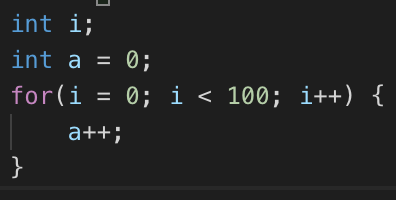
\includegraphics[width=200px]{fig1.png}
  \caption{C code snippet}
  \label{fig:fig1}
\end{figure}\\
Theoretically $a$ could be any integer value in between 1 and 100 after the code in Figure 4.1 runs. We refer to the race condition that happens between each iteration with loop-carried dependencies.\\

\begin{figure}[ht!] %
\centering
  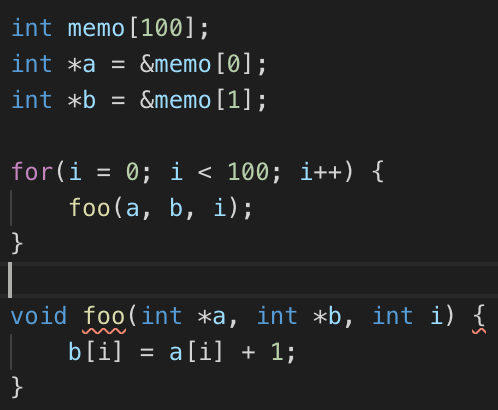
\includegraphics[width=200px]{fig2.png}
  \caption{C code snippet}
  \label{fig:fig2}
\end{figure}

Sometimes the dependency is not obvious as in Figure 4.2. At first glance one may assume $a$ and $b$ are different independent entities, while in fact they are pointing to the same piece of memory. This is called aliasing, and for automatic parallelization to work, aliasing analysis, or equivalently, pointer analysis, is required to be able to ensure that there is no dependents for computations run in parallel (which it can't assure in c).\\
\\
This brought us to the concept of parallel directives.
These tools (Open MP Pragmas) allows linear code writing to be interpreted with parallelization without the programmer having to worry about concurrency logic.
C/C++ kind of allows this sequential parallelization, but because of aliasing being allowed in the language, the correctness of results not guaranteed.
FORTRAN doesn't allow aliasing of arrays, therefore it doesn't have this issue of potential dependencies, as a result it can guarantee that the code will execute correctly if loops for example are parallelized.\\

\section{Static Analysis}
\begin{figure}[ht!] %
\centering
  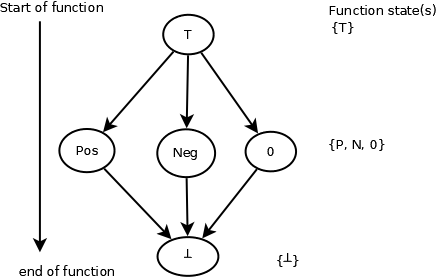
\includegraphics[width=200px]{lattice.png}
  \caption{lattice of potential states for variable x}
  \label{fig:fig3}
\end{figure}
Trying to statically analyze the code execution of program to determine potential states has multiple possible approaches: \\
\textbf{1.} Try all potential inputs to the function (possibly infinite amount of inputs to analyse)\\
\textbf{2.} Try to map the states to a more limited set of possibilities (like the figure above).\\

There are two common approaches of static code analysis: intra-procedural static analysis and inter-procedural static analysis.
\begin{table}[h!]
\begin{tabular}{|p{8cm}|p{8cm}|}
\hline
\textbf{inter-procedural} & \textbf{intra-procedural} \\ \hline
Follows/expands all function calls to evaluate those functions  & runs linearly through the function code to analyse (low runtime but state inference is less concrete)   \\ \hline
High runtime cost (potentially exponential run time) & low runtime but less potential state  inferred \\\hline
not scalable in many cases & scalable (less info though)\\\hline
\end{tabular}
\end{table}

    
\section{Branch Prediction}
We discussed the pipeline prefetching data using the fetch/decode/execute model allowing data to be loaded into higher level caches and the pipeline to reduce access time.
Then using \textbf{speculative execution}, the results from speculatively loaded instructions can be pre-computed (but hold the data back and don't commit until the branch is confirmed to be the correct branch.

Discussed CPU operation parallelization. This is called: ILP (Instruction Level Parallelizing). Unlike with loop parallelization the dependencies are able to be determined as they are all simply register addresses for the computations (if no registers in common for the operations they can be done in parallel, otherwise execute them sequentially).\\

We discussed branch prediction (to reduce time taken for loading as the instructions should already be in the pipeline (hopefully). Due to pipeline stalls/bubbles being costly in terms of computation time, we talked about the various approaches to branch prediction.\\

\large \textbf{models of prediction}:\normalsize\\
1. \textbf{Back Edge Taken}: If the loaded data is in a loop, reload the code for loop at the jump back instruction., advantages: simple, usually accurate for loops but not always (wrong if that was the last iteration of the loop).\\
2. \textbf{Last Path Taken}: Just load the data the way we did last time. This has benefits in terms of if statements. If in a loop that predictably goes down the same path, like the Back Edge Taken model though, it tends to fail when ends of loops come \\
Modern Branch Predictors need higher accuracies than the 85-95\% accuracy these simple models offer. As a result, more sophisticated models with accuracies around 99.9\% are currently used.\\
3.a. \textbf{Perceptron Branch Predictor} (used in Samsung devices)\\
3.b. \textbf{PHT (Pattern History Table)} - used in Intel\\

\section{Dynamic Memory Allocation}

\begin{figure}[ht!] %
\centering
  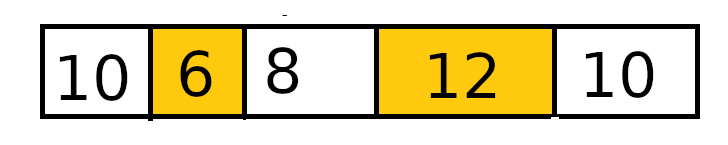
\includegraphics[width=200px]{memory_fragmentation.png}
  \caption{memory fragment, white is free}
  \label{fig:fig4}
\end{figure}

We covered dynamic memory, which is also called "heap", where we allocate objects and free them when we are done with them. We need to manage them somehow and try to reuse the freed blocks when possible. An easy way is to maintain a linked list called free list, where each node is a free block.\\

Which block should we reuse when new allocation happens? There are two different strategies we covered on this subject:\\
1. \textbf{First fit} will allocate the object to the first big enough block in free list. This method is easy and fast, but space inefficient. In Figure 4.4, we will use the first block if we allocate an object of size 8.\\
2. \textbf{Best fit}: will allocate the object to the free-block that has the smallest possible size that  will be capable of fitting the object. In Figure 4.4, we will use the third block if we allocate an object of size 8. It is easy to notice that we may need to iterate through the entire free list, which costs potential O(n) runtime, so it is time inefficient. Fragmentation can actually make this worse memory use than first fit even.\\

There is also another concern: When the memory is broken into small pieces, it is hard to reuse any of them. This is called fragmentation. We will talk more about memory management and garbage collection in the next lecture.

\end{document}
